\begin{homeworkProblem}
  aproximar una función continua $f:[0,1] \longrightarrow \mathbb{R}$ mediante un polinomio $p(t)=a_n t^n+\dots+a_1 t+a_0$,  el error de aproximación $E$ se mide en la norma $L^2$, es decir:
    \begin{align*}
        E^2:=\|p-f \|_{L^2}^2=\int_0^1[p(t)-f(t)]^2dt
    \end{align*}
  \begin{solucion}
    \begin{enumerate}[a)]
      \item Muestre que la minimización del error \( E = E(a_0, a_1, \cdots ,a_n) \) conduce a un sistema de ecuaciones lineales \( H_n a = b \), donde:
        \begin{align*}
            b = [b_0, \dots, b_n]^T \in \mathbb{R}^{n+1}, \hspace{0.3cm} b_i = \int_0^1 f(t)t^i \, dt, \hspace{1cm} i = 0, 1, \dots, n,
        \end{align*}
        \( H_n \) es la matriz de Hilbert de orden \( n \), definida como:
        \begin{align*}
            (H_n)_{i,j} = \frac{1}{i+j+1}, \hspace{1cm} i,j = 0, \cdots, n,
        \end{align*}
        y \( a \) es el vector de coeficientes de \( p \).\\
        
          Nuestro objetivo es minimizar el error en términos de los coeficientes de \( p(t) \). Para ello, simplificamos la expresión de \( E^2 \), de manera que pueda escribirse en función de \( a_0, \ldots, a_n \).
          \begin{align*}
            E^2 & := \int_0^1 [p(t) - f(t)]^2 \, dt \\
            & = \int_0^1 \left( p(t)^2 - 2p(t)f(t) + f(t)^2 \right) \, dt
          \end{align*}
          Dado que \( f(t)^2 \) no depende de \( a_i \) para \( i = 0, \cdots, n \), este término no afecta la minimización y, por lo tanto, no se considera. Así, tenemos:
          \begin{align*}
            E^2(a_0, a_1, \cdots ,a_n) = \int_0^1 p(t)^2 \, dt - 2\int_0^1 p(t)f(t) \, dt
          \end{align*}
          Como \( p(t)^2 = \left( \sum_{i=0}^n a_i t^i \right)^2 = \sum_{i=0}^n \sum_{j=0}^n a_i a_j t^{i+j} \), entonces:
          \begin{align*}
            \int_0^1 p(t)^2 \, dt = \sum_{i=0}^n \sum_{j=0}^n a_i a_j \int_0^1 t^{i+j} \, dt = \sum_{i=0}^n \sum_{j=0}^n a_i a_j \frac{1}{i+j+1}
          \end{align*}
          Además:
          \begin{align*}
            \int_0^1 p(t)f(t) \, dt & = \sum_{i=0}^n a_i \int_0^1 t^i f(t) \, dt = \sum_{i=0}^n a_i b_i, \hspace{1cm} \text{con } b_i = \int_0^1 t^i f(t) \, dt
          \end{align*}
          Sustituyendo las integrales anteriores, obtenemos:
          \begin{align*}
            E^2(a_0, a_1, \cdots ,a_n) = \sum_{i=0}^n \sum_{j=0}^n a_i a_j \frac{1}{i+j+1} - 2\sum_{i=0}^n a_i b_i
          \end{align*}
          Para minimizar \( E \), hallamos los puntos críticos resolviendo el sistema \( \nabla E^2 = \vec{0} \), lo que implica resolver:
          \begin{align*}
            \frac{\partial}{\partial a_k} \left( \sum_{i=0}^n \sum_{j=0}^n a_i a_j \frac{1}{i+j+1} - 2\sum_{i=0}^n a_i b_i \right) = 0, \hspace{0.3cm} k = 0, \cdots, n
          \end{align*}
          Calculando las derivadas parciales:
          \begin{align*}
            2\sum_{j=0}^n a_j \frac{1}{k+j+1} - 2b_k = 0
          \end{align*}
          Finalmente, el sistema de ecuaciones lineales resultante es:
          \begin{align*}
            \sum_{j=0}^n a_j \frac{1}{k+j+1} = b_k, \hspace{0.3cm} \text{con } k = 0, \cdots, n
          \end{align*}
          De forma matricial, este sistema se escribe como \( H_n a = b \):
          \[
            \begin{bmatrix}
              \frac{1}{1} & \frac{1}{2} & \cdots & \frac{1}{n+1} \\
              \frac{1}{2} & \frac{1}{3} & \cdots & \frac{1}{n+2} \\
              \vdots & \vdots & \ddots & \vdots \\
              \frac{1}{n+1} & \frac{1}{n+2} & \cdots & \frac{1}{2n+1}
            \end{bmatrix}
            \begin{bmatrix}
              a_0 \\ 
              a_1 \\ 
              \vdots \\ 
              a_n
            \end{bmatrix}
            =
            \begin{bmatrix}
              b_0 \\ 
              b_1 \\ 
              \vdots \\ 
              b_n
            \end{bmatrix}.
          \]
        \item Muestre que \( H_n \) es simétrica y definida positiva.
          Primero, demostremos que \( H_n \) es simétrica. Por definición, los elementos de \( H_n \) están dados por:
          \begin{align*}
            (H_n)_{i,j} = \frac{1}{i+j+1} = (H_n)_{j,i}, \hspace{1cm} i, j = 0, \cdots, n.
          \end{align*}
          Por lo tanto, \( H_n \) es simétrica.
          Ahora, probemos que \( H_n \) es definida positiva. Por definición, una matriz es definida positiva si, para todo vector no nulo \( \vec{x} \in \mathbb{R}^{n+1} \), se cumple que \( \vec{x}^T H_n \vec{x} > 0 \). Evaluemos:
          \begin{align*}
            \vec{x}^T H_n \vec{x} & =
            \begin{bmatrix}
              x_0 & x_1 & \cdots & x_n 
            \end{bmatrix}
            \begin{bmatrix}
              \frac{1}{1} & \frac{1}{2} & \cdots & \frac{1}{n+1} \\
              \frac{1}{2} & \frac{1}{3} & \cdots & \frac{1}{n+2} \\
              \vdots & \vdots & \ddots & \vdots \\
              \frac{1}{n+1} & \frac{1}{n+2} & \cdots & \frac{1}{2n+1}
            \end{bmatrix}
            \begin{bmatrix}
              x_0 \\ 
              x_1 \\ 
              \vdots \\ 
              x_n
            \end{bmatrix} \\
            & = \sum_{i=0}^n \sum_{j=0}^n \frac{x_i x_j}{i+j+1}.
          \end{align*}
          Observemos que:
          \begin{align*}
            \sum_{i=0}^n \sum_{j=0}^n \frac{x_i x_j}{i+j+1} &= \sum_{i=0}^n \sum_{j=0}^n x_i x_j \int_0^1 t^{i+j} \, dt \\
            &= \int_0^1 \left( \sum_{i=0}^n x_i t^i \right)^2 \, dt \\
            &= \left\| \sum_{i=0}^n x_i t^i \right\|_{L^2}^2.
          \end{align*}
          Dado que \( \left( \sum_{i=0}^n x_i t^i \right)^2 > 0 \) para cualquier \( \vec{x} \neq \vec{0} \), se cumple que:
          \begin{align*}
            \vec{x}^T H_n \vec{x} > 0.
          \end{align*}
          Por lo tanto, \( H_n \) es definida positiva.
        \item Solucione el sistema $H_nx=b$, donde b tiene componentes $b_i=1/(n+i-1)$, para $i=1, \cdots,n.$ Para esto, use las factorizaciónes LU \texttt{([L,U] = lu(H))} y Cholesky \texttt{L = chol(H);} y luego resuelva los dos sistemas triangulares, uno tras otro (es decir, realice las sustituciones hacia adelante y hacia atrás llamando al operador $\textbackslash\ $ con matrices triangulares);\\
          De forma arbitaria tomemos $n=12$, y realicemos cada uno de los pasos que se describen en el enunciado en MATLAB.
          \begin{lstlisting}[language=Matlab]
% Parametro de tamano
n = 12;  % Puedes cambiar n a cualquier valor mayor
            
% Construir la matriz de Hilbert H_n
H = zeros(n);
for c = 1:n
  for r = 1:n
    H(r,c) = 1/(r+c-1);
  end
end
            
% Construir el vector b
b = 1 ./ (n + (1:n) - 1)';  % b(i) = 1 / (n + i - 1)
            
% Factorizacion LU
[L, U] = lu(H);
            
% Resolver el sistema utilizando LU (H * x = b)
% Paso 1: Resolver L * y = b usando sustitucion hacia adelante
y = L \ b;
            
% Paso 2: Resolver U * x = y usando sustitucion hacia atras
x_LU = U \ y;
            
% Factorizaci0n de Cholesky
L_chol = chol(H, 'lower');
            
% Resolver el sistema utilizando Cholesky (H * x = b)
% Paso 1: Resolver L_chol * y = b usando sustitucion hacia adelante
y_chol = L_chol \ b;
            
% Paso 2: Resolver L_chol' * x = y usando sustitucion hacia atras
x_chol = L_chol' \ y_chol;
            
% Mostrar los resultados
disp('Solucion usando LU:');
disp(x_LU);
            
disp('Solucion usando Cholesky:');
disp(x_chol);
disp(cond(H));            
          \end{lstlisting}
          \begin{center}
            \includegraphics[scale=1]{codematlab_1.png}
            \includegraphics[scale=1.05]{codematlab_2.png}
          \end{center}
          La matriz de Hilbert es conocida por ser mal condicionada, lo que se refleja en el alto valor de su condición ($1.7086\times 10^{16}$), lo que indica que la matriz es muy sensible a pequeños errores numéricos. Este alto valor de condición causa que el método de Cholesky produzca errores significativos en las soluciones, como se observa en los valores de la solución, que están lejos de los esperados. Estos errores pueden atribuirse a la acumulación de errores de redondeo y a la inestabilidad numérica inherente en la factorización de Cholesky para matrices mal condicionadas. 
        \item Para ambos métodos ¿Qué tan precisas son la soluciones numéricas $\hat{x}_{approx}$? Tabule los errores de la solución:
        \begin{align*}
          e(n)=\|x_{approx}-x_{exact}\|
        \end{align*}
        Como una función de $n=2,\cdots, 15.$ Note que $x_{exact}=(0,\cdots,1)^T.$Puede graficar los errores en función de $n$ utilizando la función \texttt{semilogy} de Matlab. Explique en detalle los resultados.\\
          En este punto, ya habíamos demostrado que la matriz de Hilbert es definida positiva. Nuestro objetivo es analizar su comportamiento numérico al aplicarle métodos de factorización, como LU y Cholesky, para identificar las limitaciones computacionales asociadas a esta matriz.
          \begin{lstlisting}[language=matlab]
% Rango de tamaños de matriz
n_values = 2:15;
errors_LU = zeros(length(n_values), 1);
errors_Chol = zeros(length(n_values), 1);

% Calcular el error para cada tamaño de matriz
for k = 1:length(n_values)
    n = n_values(k);
    % Solución exacta (x_exact)
    x_exact = zeros(n, 1);
    x_exact(end) = 1;
    
    % Construir la matriz de Hilbert H_n
    H = zeros(n);
    for c = 1:n
        for r = 1:n
            H(r,c) = 1/(r+c-1);
        end
    end
    
    % Construir el vector b
    b = 1 ./ (n + (1:n) - 1)';  % b(i) = 1 / (n + i - 1)
    
    % Solución usando LU
    [L, U] = lu(H);
    y_LU = L \ b;
    x_LU = U \ y_LU;

    
    % Solución usando Cholesky
    L_chol = chol(H, 'lower');
    y_Chol = L_chol \ b;
    x_Chol = L_chol' \ y_Chol;
    
    % Calcular el error para LU
    errors_LU(k) = norm(x_LU - x_exact(1:n));

    % Calcular el error para Cholesky
    errors_Chol(k) =norm( x_Chol - x_exact(1:n));
 % Mostrar los errores en la tabla
    fprintf('%d\t\t%.5e\t%.5e\n', n, errors_LU(k), errors_Chol(k));
end

% Reemplazar ceros con un valor pequeño
errors_LU(errors_LU == 0) = 1e-16;
errors_Chol(errors_Chol == 0) = 1e-16;

% Graficar los errores con escala logarítmica
figure;
semilogy(n_values, errors_LU, 'b-o', 'LineWidth', 2, 'MarkerSize', 6);
hold on;
semilogy(n_values, errors_Chol, 'r-s', 'LineWidth', 2, 'MarkerSize', 6);
hold off;

% Etiquetas y título
xlabel('n (tamaño de la matriz)', 'FontSize', 13);
ylabel('Error ||x_{approx} - x_{exact}||', 'FontSize', 13);
title('Errores de la solución para diferentes tamaños n', 'FontSize', 14);
legend('LU', 'Cholesky', 'Location', 'Best');
grid on;
          \end{lstlisting}
          \begin{center}
            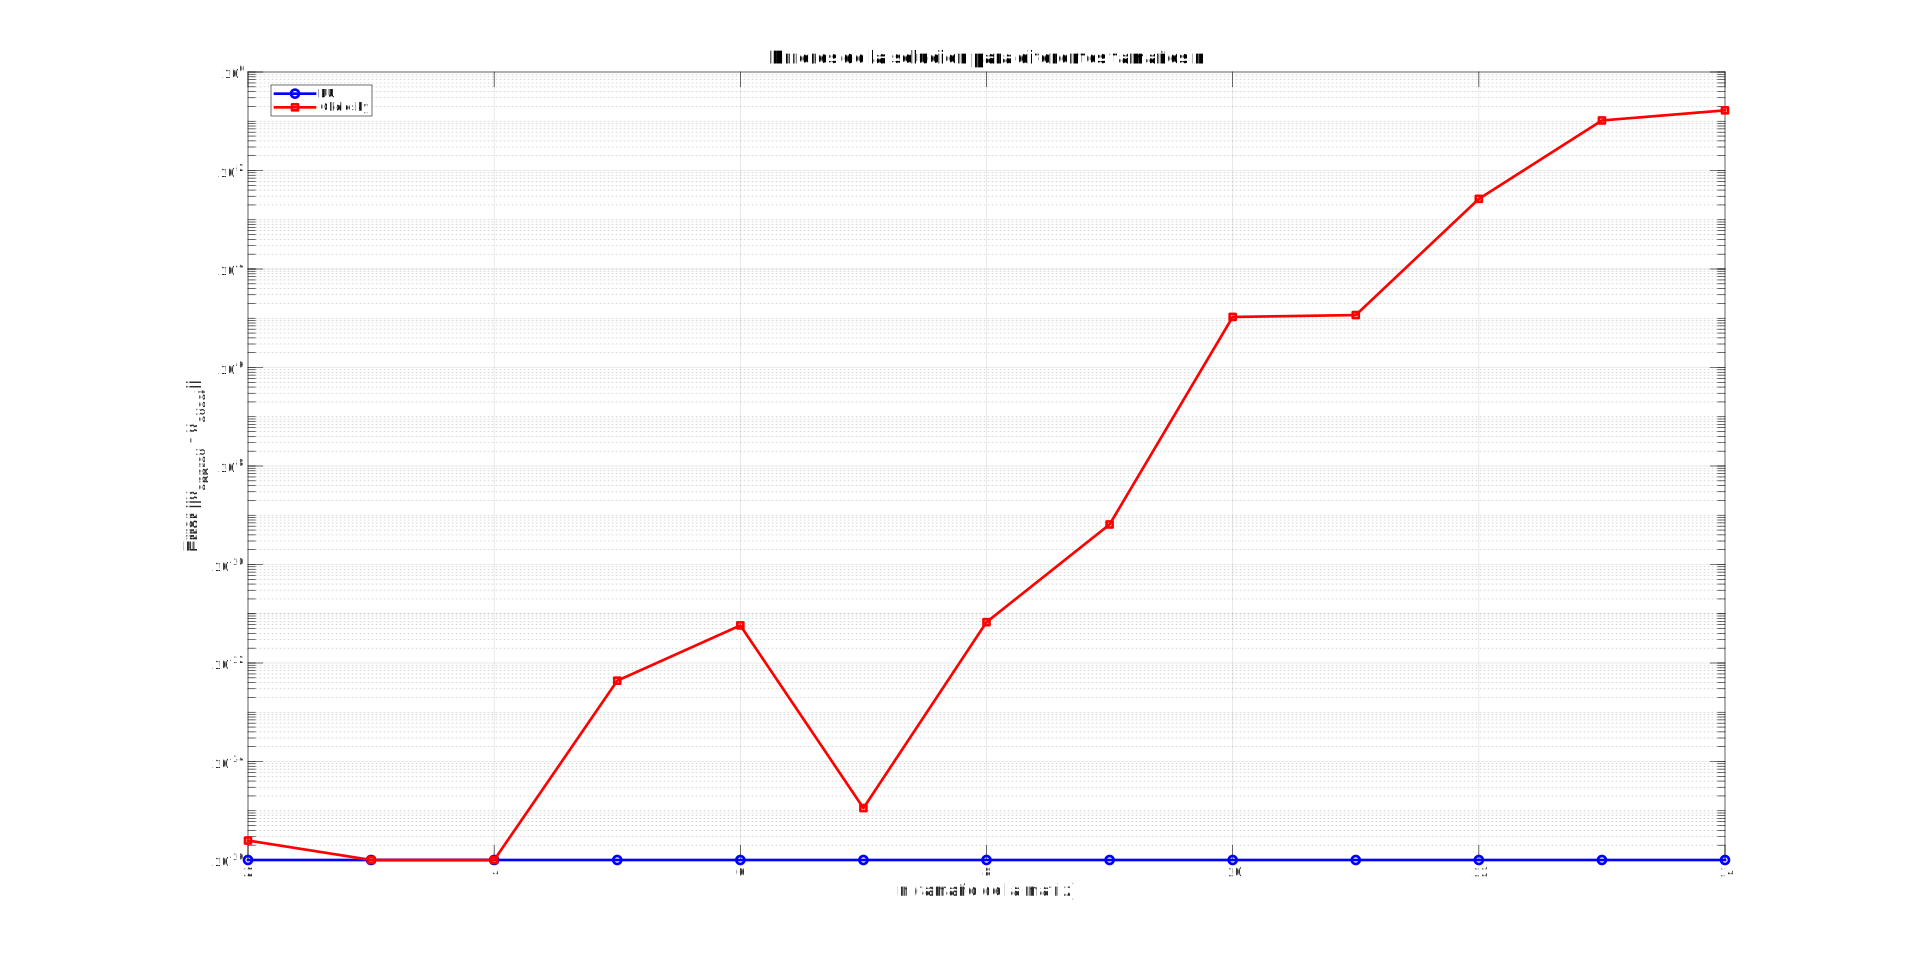
\includegraphics[scale=0.5]{grafico_matlab.jpg}\\
            \includegraphics[scale=0.6]{codematlab_4.png}
          \end{center}
          \begin{enumerate}[1)]
            \item \textbf{ Condición numérica de la matriz de Hilbert}\\
              La matriz de Hilbert \( H \) fue construida para diferentes tamaños \( n \). Esta matriz es teóricamente definida positiva y, por lo tanto, debería ser apta para la factorización de Cholesky. Sin embargo, las pruebas en MATLAB revelaron que, para valores mayores de \( n \), la función de factorización de Cholesky no puede completarse, arrojando un error indicando que la matriz no es definida positiva.
              Esto se debe a que la matriz de Hilbert es conocida por ser extremadamente mal condicionada. Esto quedó evidenciado en los cálculos del número de condición \( \kappa(H) \), el cual aumenta rápidamente con \( n \). Esta tendencia se puede observar en el siguiente algoritmo, que calcula los números de condición para \( n \) desde 2 hasta 15 y los grafica:
              \begin{lstlisting}[language=matlab]
% Cálculo y graficación del número de condición de la matriz de Hilbert
n_values = 2:15;  % Valores de n desde 2 hasta 15
cond_numbers = zeros(size(n_values));  % Vector para almacenar los números de condición
                
for i = 1:length(n_values)
  n = n_values(i);           % Tamaño de la matriz actual
  H = hilb(n);               % Generar la matriz de Hilbert
  cond_numbers(i) = cond(H); % Calcular el número de condición
end
                
% Graficar el número de condición
figure;
semilogy(n_values, cond_numbers, '-o', 'LineWidth', 1.5, 'MarkerSize', 8);
grid on;
xlabel('Tamaño de la matriz (n)', 'FontSize', 12);
ylabel('Número de condición (\kappa(H))', 'FontSize', 12);
title('Crecimiento del número de condición de la matriz de Hilbert', 'FontSize', 14);
              \end{lstlisting}
              \begin{center}
                \includegraphics[scale=0.6]{grafica.png}
              \end{center}
              \hspace{2cm}
              La gráfica generada por este código muestra cómo el número de condición \( \kappa(H) \) crece de manera significativa a medida que \( n \) aumenta, destacando la extrema sensibilidad de esta matriz a perturbaciones numéricas.
              \hspace{2cm}
            \item\textbf{ Impacto en la factorización de Cholesky} \\
              La factorización de Cholesky requiere que la matriz sea definida positiva no solo teóricamente, sino también en la práctica numérica. Durante el procedimiento, el algoritmo comprueba que los elementos diagonales de las submatrices menores sean estrictamente positivos. Sin embargo, en el caso de la matriz de Hilbert, los errores de redondeo acumulados generan perturbaciones en las entradas de \( H \), llevando a la detección de valores numéricamente no positivos en las submatrices.
              Este fenómeno se vuelve más evidente a medida que el tamaño \( n \) de la matriz aumenta, lo cual incrementa la susceptibilidad del cálculo a los errores de precisión. Como resultado, el algoritmo de Cholesky falla al interpretar \( H \) como no definida positiva.
            \item\textbf{ Comparación con la factorización LU} \\ 
              A diferencia de la factorización de Cholesky, el método de descomposición LU no tiene restricciones sobre la positividad definida de la matriz. Por esta razón, las pruebas en MATLAB mostraron que la factorización LU pudo completarse exitosamente incluso para matrices de Hilbert de tamaño grande \textbf{hasta $n\leq 25$}. Sin embargo, debido a la condición numérica extremadamente alta de \( H \), la solución obtenida mediante LU también está sujeta a errores acumulados \textbf{desde $n>25$}.\\
              \begin{lstlisting}[language=matlab]
% Parámetro de tamaño
n = 26;  % Puedes cambiar n a cualquier valor mayor

% Construir la matriz de Hilbert H_n
H = zeros(n);
for c = 1:n
    for r = 1:n
        H(r,c) = 1/(r+c-1);
    end
end

% Construir el vector b
b = 1 ./ (n + (1:n) - 1)';  % b(i) = 1 / (n + i - 1)

% Factorización LU
[L, U] = lu(H);

% Resolver el sistema utilizando LU (H * x = b)
% Paso 1: Resolver L * y = b usando sustitución hacia adelante
y = L \ b;

% Paso 2: Resolver U * x = y usando sustitución hacia atrás
x_LU = U \ y;

% Mostrar los resultados
disp('Solución usando LU:');
disp(x_LU);

disp(cond(H));
              \end{lstlisting}
              \begin{center}
                \includegraphics[scale=0.8]{lu_solution.png}  
              \end{center}
          \end{enumerate}
        \end{enumerate}         
  \end{solucion}
\end{homeworkProblem}
